% =====================================================================
%  RVCE Academic Hub -- Experiential Learning project report
%  Build:  latexmk -pdf report.tex      (or upload this folder to Overleaf)
%  Font:   Times (newtx), 12 pt, A4, 1.5 line spacing
% =====================================================================
\documentclass[12pt,a4paper,oneside]{report}

% ---------- fonts and encoding ----------
\usepackage[T1]{fontenc}
\usepackage[utf8]{inputenc}
\usepackage{newtxtext,newtxmath}   % Times New Roman for text and mathematics

% ---------- page layout ----------
\usepackage[a4paper,top=1in,bottom=1in,left=1.25in,right=1in,headheight=15pt]{geometry}
\usepackage{setspace}
\onehalfspacing
\usepackage{fancyhdr}
\usepackage{titlesec}
\usepackage{enumitem}
\setlist{itemsep=2pt,topsep=4pt}

% ---------- tables, figures, code ----------
\usepackage{graphicx}
\usepackage{booktabs}
\usepackage{tabularx}
\usepackage{longtable}
\usepackage{array}
\usepackage{xcolor}
\usepackage{caption}
\captionsetup{font=small,labelfont=bf,skip=6pt}
\usepackage{listings}
\usepackage{tikz}
\usetikzlibrary{positioning,arrows.meta,fit,shapes.geometric}
\usepackage[hidelinks]{hyperref}

% ---------- colours (match the application) ----------
\definecolor{brand}{HTML}{2E9DFF}
\definecolor{brandstrong}{HTML}{126CDE}
\definecolor{ink}{HTML}{0B1220}
\definecolor{soft}{HTML}{E8F3FF}
\definecolor{codebg}{HTML}{F5F8FC}
\definecolor{codekw}{HTML}{126CDE}
\definecolor{codestr}{HTML}{10915E}
\definecolor{codecom}{HTML}{8897AD}

% ---------- headings ----------
\titleformat{\chapter}[display]
  {\normalfont\bfseries\centering}
  {\large\MakeUppercase{\chaptertitlename}~\thechapter}{6pt}{\Large\MakeUppercase}
\titlespacing*{\chapter}{0pt}{0pt}{24pt}
\titleformat{\section}{\normalfont\large\bfseries}{\thesection}{1em}{}
\titleformat{\subsection}{\normalfont\normalsize\bfseries}{\thesubsection}{1em}{}

% ---------- header / footer ----------
\pagestyle{fancy}
\fancyhf{}
\fancyhead[L]{\small RVCE Academic Hub}
\fancyhead[R]{\small\nouppercase{\leftmark}}
\fancyfoot[C]{\small\thepage}
\renewcommand{\headrulewidth}{0.4pt}
\fancypagestyle{plain}{\fancyhf{}\fancyfoot[C]{\small\thepage}\renewcommand{\headrulewidth}{0pt}}

% ---------- helpers ----------
\newcommand{\TODO}[1]{\textcolor{red}{[#1]}}
\newcommand{\code}[1]{\texttt{\detokenize{#1}}}
\newcommand{\appname}{RVCE Academic Hub}
% \fig{file}{caption}{label}{width}: never breaks the build if an image is missing
\newcommand{\fig}[4]{%
  \begin{figure}[htbp]\centering
    \IfFileExists{figures/#1}%
      {\includegraphics[width=#4\linewidth]{figures/#1}}%
      {\fbox{\parbox[c][4cm][c]{0.8\linewidth}{\centering\small Figure file \texttt{figures/#1} not found}}}%
    \caption{#2}\label{#3}
  \end{figure}}

\lstdefinelanguage{JavaScript}{
  keywords={const,let,var,function,return,if,else,for,of,in,new,async,await,export,import,from,throw,true,false,null,undefined},
  sensitive=true,
  comment=[l]{//}, morecomment=[s]{/*}{*/},
  string=[b]', morestring=[b]", morestring=[b]`}
\lstdefinelanguage{plain}{}
\lstset{
  language=JavaScript, basicstyle=\ttfamily\footnotesize, backgroundcolor=\color{codebg},
  keywordstyle=\color{codekw}\bfseries, stringstyle=\color{codestr}, commentstyle=\color{codecom}\itshape,
  frame=single, rulecolor=\color{soft}, framesep=6pt, xleftmargin=8pt, xrightmargin=8pt,
  breaklines=true, columns=fullflexible, keepspaces=true, showstringspaces=false,
  numbers=left, numberstyle=\tiny\color{codecom}, numbersep=6pt, aboveskip=10pt, belowskip=10pt}

\hypersetup{pdftitle={RVCE Academic Hub: Experiential Learning Report},pdfauthor={RVCE Academic Hub team}}

% =====================================================================
\begin{document}

% ---------------------------------------------------------------------
%  Title page
% ---------------------------------------------------------------------
\begin{titlepage}
  \centering
  {\large\bfseries R V COLLEGE OF ENGINEERING\par}
  {\small (Autonomous Institution Affiliated to Visvesvaraya Technological University, Belagavi)\par}
  {\small Bengaluru -- 560059\par}
  \vspace{1.2cm}
  {\large Department of \TODO{Computer Science and Engineering}\par}
  \vspace{1.5cm}
  {\normalsize EXPERIENTIAL LEARNING REPORT\par}
  {\normalsize on\par}
  \vspace{0.6cm}
  {\LARGE\bfseries \appname\par}
  \vspace{0.3cm}
  {\large A Full-Stack Platform for Proctored Quizzes,\\ Live Monitoring and Results\par}
  \vspace{1.5cm}
  {\normalsize Submitted in partial fulfilment of the course\par}
  {\normalsize\bfseries Full Stack Application Development \TODO{(Course code)}\par}
  \vspace{1.2cm}
  {\normalsize Submitted by\par}
  \vspace{0.3cm}
  \begin{tabular}{ll}
    \TODO{Student name 1} & \TODO{USN} \\
    \TODO{Student name 2} & \TODO{USN} \\
    \TODO{Student name 3} & \TODO{USN} \\
  \end{tabular}
  \vspace{1.2cm}

  {\normalsize Under the guidance of\par}
  {\normalsize\bfseries \TODO{Guide name}\par}
  {\normalsize \TODO{Designation}, Department of \TODO{CSE}\par}
  \vfill
  {\normalsize Academic Year \TODO{2026--27}\par}
\end{titlepage}

\pagenumbering{roman}

% ---------------------------------------------------------------------
\chapter*{Certificate}
\addcontentsline{toc}{chapter}{Certificate}
This is to certify that the Experiential Learning project titled \textbf{``\appname''} has been carried out by
\TODO{Student names and USNs}, bona fide students of R V College of Engineering, Bengaluru, in partial fulfilment
of the requirements of the course \textbf{Full Stack Application Development} during the academic year
\TODO{2026--27}. The project report has been approved as it satisfies the academic requirements prescribed for the course.

\vspace{3cm}
\noindent
\begin{tabularx}{\linewidth}{@{}X X@{}}
  \rule{5cm}{0.4pt} & \rule{5cm}{0.4pt} \\
  Signature of the Guide & Signature of the Head of Department \\
  \TODO{Guide name} & \TODO{HoD name} \\
\end{tabularx}

% ---------------------------------------------------------------------
\chapter*{Declaration}
\addcontentsline{toc}{chapter}{Declaration}
We, the students of the Department of \TODO{Computer Science and Engineering}, R V College of Engineering, Bengaluru,
declare that the Experiential Learning project titled \textbf{``\appname''} has been carried out by us and submitted
in partial fulfilment of the course Full Stack Application Development. The work presented in this report is original
and has not been submitted elsewhere for the award of any degree or credit.

\vspace{2cm}
\noindent Place: Bengaluru \hfill \TODO{Student names and signatures}\\
Date: \TODO{date}

% ---------------------------------------------------------------------
\chapter*{Acknowledgement}
\addcontentsline{toc}{chapter}{Acknowledgement}
We thank our guide, \TODO{Guide name}, for the direction and feedback given throughout this project. We thank the
Head of the Department, \TODO{HoD name}, and the Principal of R V College of Engineering for providing the facilities
and the opportunity to carry out this Experiential Learning work. We also thank the faculty members and our classmates
who tried the application and reported issues during testing.

% ---------------------------------------------------------------------
\chapter*{Abstract}
\addcontentsline{toc}{chapter}{Abstract}
Short, frequent quizzes help students retain material, but running them online raises three practical problems for a
department: conducting them fairly when students sit in front of their own browsers, giving teachers a live view of
what is happening during the quiz, and turning the results into records that can be published, reviewed and exported.

\appname{} is a full-stack web application built with MongoDB, Express, React and Node.js (MERN) that addresses these
problems for a college department. Administrators manage the academic structure and allocate subjects; teachers build
fixed 10-mark quizzes from a question bank, schedule them or run them in a live room, and watch every attempt on a live
monitor; students write the quiz on a distraction-free, proctored exam screen with a server-synchronised timer and
automatic saving. Browser-level proctoring records tab switches, focus loss, fullscreen exits and duplicate tabs,
merges events caused by a single action, and submits an attempt automatically when the teacher's warning limit is
reached. Results are scored automatically, published by the teacher, and reviewed question by question by the student;
teachers and administrators can export results as CSV files or Excel workbooks.

The interface follows a consistent design system inspired by a modern quiz-application concept, using a single brand
colour (\#2E9DFF), accessible contrast, dark mode and layouts that work on phones. The server is covered by automated
unit tests for scoring, proctoring rules, CSV parsing and the export format, and the complete student and teacher flows
were exercised end to end in a browser.

\noindent\textbf{Keywords:} MERN stack, online assessment, browser proctoring, Socket.IO, real-time monitoring,
automatic grading, data export.

% ---------------------------------------------------------------------
\tableofcontents
\listoffigures
\listoftables

\cleardoublepage
\pagenumbering{arabic}

% =====================================================================
\chapter{Introduction}
\label{ch:intro}

\section{Background}
Continuous internal evaluation in engineering colleges relies on many small assessments: quizzes, assignments and
tests spread across the semester. Paper quizzes are slow to mark and hard to analyse, while generic online form tools
are easy to set up but give teachers no control over the exam environment and no live view of who is writing, who has
left the page or who has disconnected. Results also tend to stay inside the tool, so teachers re-type marks into
spreadsheets before they can be consolidated.

\section{Problem statement}
Design and implement a web application that lets a department run short online quizzes end to end: from building a
question paper, through a fair and monitored attempt, to publishing results that students can review and teachers can
export, while keeping the experience simple enough for students to use on any device.

\section{Objectives}
\begin{enumerate}
  \item Provide role-based access for administrators, teachers and students, restricted to pre-provisioned institutional accounts.
  \item Let teachers build quizzes worth exactly 10 marks from multiple-choice and single-line fill-in questions, and schedule them or run them in a live room.
  \item Give students a distraction-free exam screen with a server-synchronised timer, automatic saving and recovery from network loss.
  \item Detect and record browser-level integrity events, apply a configurable warning policy, and submit automatically at the limit.
  \item Give teachers a live monitor with per-student progress, warnings and controls (pause, resume, end, message, extend time, force submit).
  \item Score attempts automatically, let teachers publish results, and let students review every answer once results are published.
  \item Export results as CSV and Excel files for record keeping.
\end{enumerate}

\section{Scope}
The application covers academic structure (departments, years, semesters, sections, subjects and allocations), the
quiz life cycle, proctoring, live monitoring, grading, publication, grade review requests, assignments, announcements,
notifications and an academic calendar. Quizzes are deliberately limited to two auto-markable question types and a
fixed total of 10 marks so that results are comparable across subjects. Camera, microphone or screen recording are
outside the scope: proctoring is limited to signals the browser exposes, which keeps the system light and respects
student privacy.

\section{Organisation of the report}
Chapter~\ref{ch:req} lists the requirements. Chapter~\ref{ch:design} presents the architecture, data model and
interfaces. Chapter~\ref{ch:impl} describes the implementation of each module. Chapter~\ref{ch:test} reports testing
and results, and Chapter~\ref{ch:concl} concludes with future work. Appendix~\ref{app:run} explains how to run the
project and Appendix~\ref{app:api} lists the API endpoints.

% =====================================================================
\chapter{Requirements}
\label{ch:req}

\section{Users and roles}
\begin{description}
  \item[Administrator] manages users (including bulk CSV import), the academic structure, subject allocations, audit logs and institution-wide reports.
  \item[Teacher] manages the question bank and quizzes for allocated subjects, runs and monitors quizzes, evaluates and publishes results, and answers grade review requests.
  \item[Student] writes quizzes for enrolled subjects, views published results with a per-question review, requests clarification on a mark, and downloads their grades.
\end{description}

\section{Functional requirements}
\begin{longtable}{@{}p{0.09\linewidth}p{0.86\linewidth}@{}}
\caption{Functional requirements}\label{tab:fr}\\
\toprule
\textbf{ID} & \textbf{Requirement}\\ \midrule
\endfirsthead
\toprule
\textbf{ID} & \textbf{Requirement}\\ \midrule
\endhead
FR1 & Users sign in with an institutional Google account; only pre-provisioned, approved accounts are admitted. A development-only sign-in picker can be enabled locally.\\
FR2 & Each request is authorised by role and, for teachers, by allocation to the subject concerned.\\
FR3 & Teachers create questions (single-correct MCQ or single-line fill-in) with marks in steps of 0.5, difficulty, topic and explanation.\\
FR4 & A quiz can be saved only when its questions total exactly 10 marks; drafts can be edited until published.\\
FR5 & A quiz is available on a schedule, immediately on publish, or in a live room that students join with a code.\\
FR6 & Proctoring is configurable per quiz: fullscreen, clipboard and context-menu blocking, duplicate-tab and developer-tool detection, and a warning limit.\\
FR7 & The exam screen shows one question at a time with a question palette, mark-for-review, a countdown and a submit summary; answers save automatically.\\
FR8 & Integrity events are recorded on the server; warnings that reach the limit submit the attempt automatically.\\
FR9 & Teachers see a live roster with status, progress, warnings and time left, and can pause, resume or end the quiz, message a student, add time or force-submit.\\
FR10 & Attempts are scored automatically; the best attempt is kept as the grade; teachers publish grades individually or all at once.\\
FR11 & After publication, students see their score and a per-question review; they may request a review of a mark.\\
FR12 & Teachers export a quiz's results, students export their own grades and administrators export all published grades, as CSV or Excel.\\
\bottomrule
\end{longtable}

\section{Non-functional requirements}
\begin{itemize}
  \item \textbf{Integrity:} time limits are enforced on the server; correct answers never reach the browser before results are published.
  \item \textbf{Reliability:} answers survive a page reload or a temporary network loss; reconnecting resumes the attempt.
  \item \textbf{Responsiveness:} live monitor updates arrive within about a second over WebSockets.
  \item \textbf{Usability and accessibility:} a consistent design system, keyboard navigation in the exam, visible focus, sufficient text contrast, dark mode and layouts that work at 390\,px width.
  \item \textbf{Security:} HTTP-only session cookies, Helmet security headers, rate limiting on authentication, input validation with Zod, audit logging of administrative actions, and protection against spreadsheet formula injection in exports.
  \item \textbf{Maintainability:} a modular server, shared UI components, automated tests and a one-command local runner.
\end{itemize}

\section{Hardware and software requirements}
\begin{table}[htbp]\centering
\caption{Development and runtime environment}\label{tab:env}
\begin{tabularx}{\linewidth}{@{}lX@{}}
\toprule
\textbf{Item} & \textbf{Requirement}\\ \midrule
Processor / memory & Any x86-64 or ARM64 machine with 4\,GB RAM or more\\
Operating system & Linux, macOS or Windows (WSL for the shell script)\\
Runtime & Node.js 20 or later, npm\\
Database & MongoDB 7 (local \code{mongod} or Docker)\\
Browser & A current Chromium, Firefox or Safari with the Fullscreen API\\
Tools & Git, a code editor, optionally Docker Compose\\
\bottomrule
\end{tabularx}
\end{table}

% =====================================================================
\chapter{System Design}
\label{ch:design}

\section{Architecture}
The system is a modular monolith in one npm workspace with two applications (Figure~\ref{fig:arch}). The React client
talks to the Express API over HTTPS using JSON and an HTTP-only session cookie, and to the Socket.IO server over a
WebSocket for real-time events. The API is the only component that accesses MongoDB.

\begin{figure}[htbp]\centering
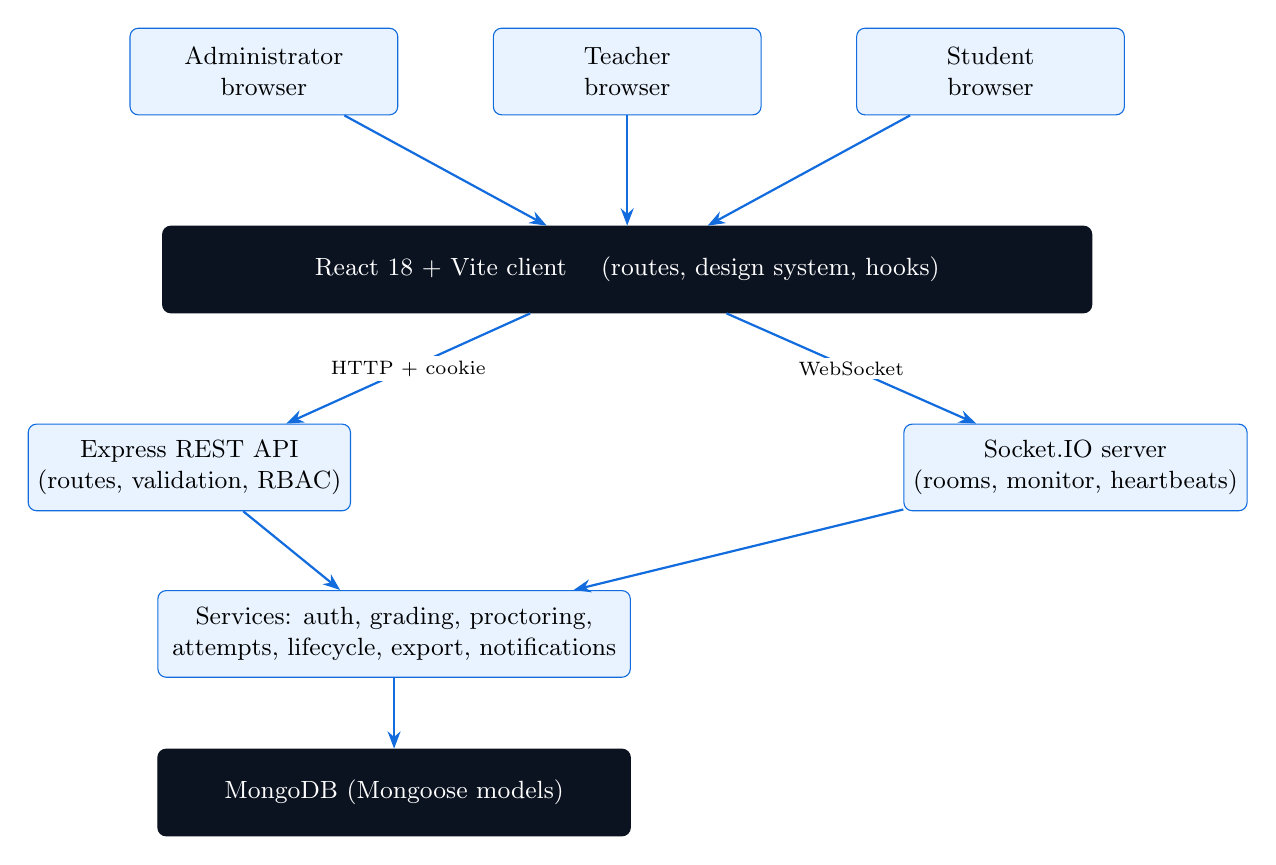
\begin{tikzpicture}[
  node distance=9mm and 12mm,
  box/.style={draw=brandstrong, fill=soft, rounded corners=3pt, align=center, minimum width=34mm, minimum height=11mm, font=\small},
  dark/.style={box, draw=ink, fill=ink, text=white},
  arr/.style={-{Stealth[length=2.2mm]}, thick, draw=brandstrong},
  lbl/.style={font=\scriptsize, fill=white, inner sep=1.5pt}]
  \node[box] (admin) {Administrator\\browser};
  \node[box, right=of admin] (teacher) {Teacher\\browser};
  \node[box, right=of teacher] (student) {Student\\browser};
  \node[dark, below=14mm of teacher, minimum width=118mm] (client) {React 18 + Vite client \quad (routes, design system, hooks)};
  \node[box, below left=14mm and -24mm of client] (api) {Express REST API\\(routes, validation, RBAC)};
  \node[box, below right=14mm and -24mm of client] (io) {Socket.IO server\\(rooms, monitor, heartbeats)};
  \node[box, below=10mm of api, xshift=26mm, minimum width=60mm] (svc) {Services: auth, grading, proctoring,\\attempts, lifecycle, export, notifications};
  \node[dark, below=9mm of svc, minimum width=60mm] (db) {MongoDB (Mongoose models)};
  \foreach \u in {admin,teacher,student} \draw[arr] (\u) -- (client);
  \draw[arr] (client) -- node[lbl]{HTTP + cookie} (api);
  \draw[arr] (client) -- node[lbl]{WebSocket} (io);
  \draw[arr] (api) -- (svc);
  \draw[arr] (io) -- (svc);
  \draw[arr] (svc) -- (db);
\end{tikzpicture}
\caption{High-level architecture}\label{fig:arch}
\end{figure}

\section{Technology stack}
\begin{table}[htbp]\centering
\caption{Technology stack}\label{tab:stack}
\begin{tabularx}{\linewidth}{@{}lX@{}}
\toprule
\textbf{Layer} & \textbf{Technology and purpose}\\ \midrule
User interface & React 18, React Router 6, Tailwind CSS 3 with CSS-variable design tokens, lucide icons, Recharts\\
Forms & react-hook-form with Zod schemas shared in spirit with the server\\
Client build & Vite 6\\
Real time & Socket.IO 4 (client and server)\\
Server & Node.js 20+, Express 4, Helmet, CORS, express-rate-limit, cookie-parser\\
Validation & Zod\\
Authentication & Google Identity Services, google-auth-library, JSON Web Tokens in HTTP-only cookies\\
Database & MongoDB 7 with Mongoose 8\\
Exports & ExcelJS (XLSX) and a small RFC~4180 CSV writer\\
Testing & Node.js built-in test runner, Supertest\\
Tooling & ESLint, Prettier, Docker Compose, \code{run.sh}\\
\bottomrule
\end{tabularx}
\end{table}

\section{Module decomposition}
\begin{itemize}
  \item \textbf{Identity and access:} Google sign-in, development sign-in, session cookies, role checks and subject-level authorisation.
  \item \textbf{Academic structure:} departments, academic years, semesters, sections, subjects, teacher assignments and enrolments.
  \item \textbf{Question bank and quiz builder:} question CRUD with usage locks, five-step quiz builder, publication.
  \item \textbf{Exam engine:} start or resume, paper shuffling, server timing, autosave, submission and finalisation.
  \item \textbf{Proctoring:} event capture in the browser, server-side classification and warning policy.
  \item \textbf{Live monitoring:} socket rooms per quiz, roster snapshot, progress, presence and teacher controls.
  \item \textbf{Results:} automatic scoring, grade publication, per-question review, review requests and exports.
  \item \textbf{Communication:} notifications, announcements and calendar events.
\end{itemize}

\section{Data model}
MongoDB stores one document per entity; relationships are object-id references resolved with Mongoose
\code{populate}. Table~\ref{tab:collections} lists the collections central to the quiz flow.

\begin{longtable}{@{}>{\raggedright\arraybackslash}p{0.2\linewidth}>{\raggedright\arraybackslash}p{0.75\linewidth}@{}}
\caption{Main collections and key fields}\label{tab:collections}\\
\toprule
\textbf{Collection} & \textbf{Key fields}\\ \midrule
\endfirsthead
\toprule
\textbf{Collection} & \textbf{Key fields}\\ \midrule
\endhead
User & name, email, role (admin, teacher, student), USN, department, active and approval status\\
Subject & code, name, department, semester, academic year, credits, coordinator, teachers[], students[]\\
Question & subject, creator, text, type (single, fill\_blank), topic, difficulty, marks, options[\{key, text\}], correctAnswer, explanation\\
Assessment & subject, creator, title, state (DRAFT, SCHEDULED, AVAILABLE, LIVE, PAUSED, ENDED, PUBLISHED, \dots), questionIds[], maxMarks (10), durationMinutes, startsAt, endsAt, availabilityMode, attemptsAllowed, shuffle flags, proctoring policy, pausedAt\\
Attempt & assessment, student, attemptNumber, questionOrder[], optionOrders[], answers[\{question, value, flagged, savedAt\}], state, startedAt, deadlineAt, submittedAt, submitReason, score, violationCount, proctoringEvents[], lastSeenAt\\
Grade & assessment, student, attempt, rawMarks, maxMarks, feedback, publishedAt\\
GradeReviewRequest & grade, student, message, status (OPEN, APPROVED, REJECTED), response\\
Room & code, assessment, teacher, status, eligibleStudents[], participants[], expiresAt\\
Notification, AuditLog & recipient, title, body, link; actor, action, entity, details\\
\bottomrule
\end{longtable}

\noindent A unique index on \code{(assessment, student, attemptNumber)} prevents duplicate attempts, and a unique
index on \code{(assessment, student)} keeps exactly one grade per student and quiz.

\section{Interfaces}
\subsection{REST API}
All responses use the envelope \texttt{\{ ok, data \}} or \texttt{\{ ok: false, error \}}. Table~\ref{tab:api-core} lists
the endpoints of the quiz flow; the complete list is in Appendix~\ref{app:api}.

\begin{table}[htbp]\centering
\caption{Core quiz endpoints}\label{tab:api-core}
\small
\begin{tabularx}{\linewidth}{@{}l>{\raggedright\arraybackslash}p{0.42\linewidth}X@{}}
\toprule
\textbf{Method} & \textbf{Path} & \textbf{Purpose}\\ \midrule
POST & \code{/assessments} & Create a quiz (optionally publish)\\
POST & \code{/assessments/:id/start} & Start or resume an attempt (student)\\
PATCH & \code{/attempts/:id/answers} & Autosave one answer\\
POST & \code{/attempts/:id/proctoring-events} & Record an integrity event\\
POST & \code{/attempts/:id/submit} & Submit the attempt\\
GET & \code{/assessments/:id/monitor} & Live roster and recent events (teacher)\\
POST & \code{/assessments/:id/pause}, \code{resume}, \code{end} & Quiz controls\\
POST & \code{/grades/:id/publish} & Publish one result\\
GET & \code{/assessments/:id/my-result} & Per-question review after publication\\
GET & \code{/assessments/:id/results.csv}, \code{.xlsx} & Export quiz results\\
\bottomrule
\end{tabularx}
\end{table}

\subsection{Real-time events}
\begin{table}[htbp]\centering
\caption{Socket.IO events}\label{tab:events}
\small
\begin{tabularx}{\linewidth}{@{}l l X@{}}
\toprule
\textbf{Direction} & \textbf{Event} & \textbf{Meaning}\\ \midrule
Client $\rightarrow$ server & \code{monitor:join}, \code{monitor:leave} & Teacher subscribes to a quiz's monitor room\\
Client $\rightarrow$ server & \code{attempt:heartbeat} & Student is still connected (every 15 s)\\
Client $\rightarrow$ server & \code{room:join}, \code{room:start} & Live room lobby and start\\
Server $\rightarrow$ teacher & \code{monitor:progress}, \code{monitor:presence} & Answered count, online or offline\\
Server $\rightarrow$ teacher & \code{monitor:submitted}, \code{proctor:event} & Submission with score; integrity event\\
Server $\rightarrow$ teacher & \code{monitor:state}, \code{monitor:extended} & Quiz state change; extra time\\
Server $\rightarrow$ student & \code{assessment:paused}, \code{resumed}, \code{ended} & Quiz controls applied live\\
Server $\rightarrow$ student & \code{attempt:message}, \code{extended}, \code{force-submitted} & Teacher actions on one attempt\\
\bottomrule
\end{tabularx}
\end{table}

\section{Attempt life cycle}
\begin{enumerate}
  \item The student opens the quiz; the rules screen lists the active proctoring policy and asks for consent.
  \item On \emph{Start}, the browser enters fullscreen and calls \code{/start}. The server creates the attempt, fixes a shuffled question order and per-question option order, and sets \code{deadlineAt}.
  \item The client synchronises its clock to the server time in the response; every answer is saved immediately (choices) or after 600 ms (text).
  \item Integrity events are posted to the server, which classifies them and returns the updated warning count.
  \item The attempt ends by manual submission, timeout, the teacher ending the quiz, a forced submission, or the warning limit. In every case the server scores the paper and updates the grade.
  \item After the teacher publishes the grade, the student can open the per-question review.
\end{enumerate}

% =====================================================================
\chapter{Implementation}
\label{ch:impl}

\section{Authentication and authorisation}
Users sign in with Google Identity Services. The server verifies the ID token with google-auth-library, checks the
allowed domain (\code{rvce.edu.in} by default) and requires the account to exist, be active and be approved. A signed
JWT is stored in an HTTP-only, SameSite=Lax cookie. Middleware \code{authenticate} loads the user on each request and
\code{allow(...roles)} rejects other roles; teacher routes also check that the teacher is allocated to the subject.
For local development a sign-in picker can be enabled with \code{DEV_LOGIN=true}; it is ignored when
\code{NODE_ENV=production}. Authentication routes are rate limited.

\section{Question bank and quiz builder}
Questions are edited in a drawer with structured option rows, click-to-mark correct answer, marks in 0.5 steps and a
live student preview. The quiz builder is a five-step form (details, questions, schedule, proctoring, review) built
with react-hook-form and Zod. A ring-shaped meter shows the running total and blocks progress until it is exactly 10;
the server repeats the check in \code{checkPaper} so the rule cannot be bypassed. The review step previews the quiz
card exactly as students will see it.

\section{Exam engine}
The exam page has four phases: gate (rules and consent), exam, finished and duplicate tab. Important properties:
\begin{itemize}
  \item \textbf{Server-authoritative time.} The deadline lives on the attempt; the client corrects its clock using the server time returned with each payload, and a background job submits expired attempts. Pausing a quiz freezes the remaining time and resuming moves the deadline.
  \item \textbf{Autosave and recovery.} One request per question is in flight at a time; answers are mirrored to local storage, survive a reload, and are retried when the browser comes back online.
  \item \textbf{No answer leakage.} The exam payload contains question text and options only; correct answers are never sent to the browser while the attempt is active.
\end{itemize}

\section{Proctoring}
\code{useProctoring} listens for visibility changes, window blur, fullscreen exit, a second tab (BroadcastChannel),
offline periods and blocked shortcuts. The server service \code{proctoring.js} classifies each event as
\emph{critical}, \emph{warning} or \emph{info}. A single tab switch usually fires blur, visibility and fullscreen events
together, so events of the focus-loss family within 1.5 seconds are merged into one incident. Only counted incidents
increase the warning count; when it reaches the quiz's limit the attempt is finalised with the reason
\code{PROCTORING_LIMIT}. The student sees a blocking overlay that explains the event and the warnings left.

\section{Live monitor}
When a teacher opens the monitor, the client emits \code{monitor:join}; the server confirms that the teacher may
monitor the quiz and adds the socket to the room \code{monitor:<quizId>}. The page combines an initial snapshot from
\code{/monitor} with incremental socket events, so it stays correct after reconnection. It shows stat cards, a
filterable roster with status, progress, warnings and time left, a live activity feed and a per-student timeline, and
offers pause, resume, end, message, extra time and force submit. After the quiz ends, the same page becomes a report
with the average score and a podium of the top three students (Figure~\ref{fig:report}).

\section{Grading, publication and review}
\code{finalizeAttempt} submits an attempt exactly once using an atomic conditional update, scores it with
\code{evaluateObjective}, and keeps the best score in the student's grade. Fill-in answers are compared after trimming
and ignoring case. Grades stay private until the teacher publishes them. The student result endpoint returns the
per-question breakdown only for a published grade; the breakdown is produced by \code{reviewAnswers}
(Listing~\ref{lst:review}).

\begin{lstlisting}[caption={Per-question review used by the student and teacher result pages},label={lst:review}]
export function reviewAnswers(questions, answers = []) {
  return questions.map((q) => {
    const answer = answers.find((item) => String(item.question) === String(q._id));
    const given = isBlank(answer?.value) ? null : answer.value;
    const right = given !== null && sameAnswer(given, q.correctAnswer);
    return {
      id: String(q._id), text: q.text, type: q.type, marks: q.marks,
      options: (q.options || []).map(({ key, text }) => ({ key, text })),
      correctAnswer: q.correctAnswer, explanation: q.explanation, given,
      status: given === null ? 'skipped' : right ? 'correct' : 'incorrect',
      awarded: right ? q.marks : 0,
      flagged: Boolean(answer?.flagged),
    };
  });
}
\end{lstlisting}

\section{Exporting results}
Results can be downloaded in two formats from the Evaluation page, the quiz report, \emph{My grades} and the
administrator dashboard (Figure~\ref{fig:export}).
\begin{itemize}
  \item \textbf{CSV} follows RFC~4180, starts with a UTF-8 byte-order mark so spreadsheet applications read names correctly, quotes every cell and uses CRLF line endings.
  \item \textbf{Excel (XLSX)} is generated with ExcelJS. A quiz workbook has three sheets: \emph{Results} (one row per enrolled student with status, score, percentage, correct, incorrect and skipped counts, warnings, submission reason and timings), \emph{Question breakdown} (marks awarded per question) and \emph{Summary} (enrolment, submissions, average, highest and lowest). Headers are bold, tinted, frozen and filterable; percentages and dates use native number formats.
  \item \textbf{Formula injection.} Any text cell that starts with \code{=}, \code{+}, \code{-}, \code{@} or a tab is prefixed with an apostrophe so a spreadsheet never evaluates student-supplied text as a formula.
\end{itemize}

\begin{lstlisting}[caption={CSV cells are neutralised before quoting},label={lst:csv}]
const FORMULA_START = /^[=+\-@\t\r]/;
export function safeCell(value) {
  if (value === null || value === undefined) return '';
  if (value instanceof Date) return value.toISOString();
  if (typeof value === 'number' || typeof value === 'boolean') return String(value);
  const text = String(value);
  return FORMULA_START.test(text) ? `'${text}` : text;
}
\end{lstlisting}

\section{User interface and design system}
The interface was redesigned after a contemporary quiz-application concept and adapted to the institution's needs.
\begin{itemize}
  \item \textbf{Tokens.} All colours are CSS variables consumed by Tailwind, with separate light and dark values. The brand colour \#2E9DFF is used for fills, rings and progress; a darker tone (\#126CDE) is used for text and buttons with white labels so contrast stays readable.
  \item \textbf{Components.} Gradient ``hero'' cards with a fading dot texture, black call-to-action pills tucked into a card corner, small uppercase chips, number pills, section titles with a dot bullet, timer and score rings, segmented tabs and a stepper.
  \item \textbf{Student experience.} A home page with the next quiz, progress ring and subject tiles; a quiz list as cards; an exam screen with a sticky header, countdown ring and large option rows; and a result page where correct options are shown in green and wrong choices in red.
  \item \textbf{Accessibility.} Keyboard navigation between questions, visible focus rings, ARIA labels on icon buttons and the timer, reduced-motion support and layouts that fit a 390\,px screen.
  \item \textbf{Typography.} Poppins for headings and numbers, DM Sans for body text.
\end{itemize}

\section{Developer experience}
\code{run.sh} starts the whole system with one command. On the first run it creates a local \code{.env} with a random
JWT secret, installs dependencies, starts MongoDB (a local \code{mongod} with data in \code{.data/}, or Docker
Compose), seeds sample data when the database is empty, and runs the API and the client together. It also offers
\code{setup}, \code{seed}, \code{test}, \code{build} and \code{stop} commands (Appendix~\ref{app:run}).

% =====================================================================
\chapter{Testing and Results}
\label{ch:test}

\section{Automated tests}
Server tests use the Node.js test runner and Supertest. All 20 tests pass (Table~\ref{tab:tests}).

\begin{table}[htbp]\centering
\caption{Automated test suites}\label{tab:tests}
\small
\begin{tabularx}{\linewidth}{@{}l c X@{}}
\toprule
\textbf{Suite} & \textbf{Tests} & \textbf{What is verified}\\ \midrule
\code{proctoring.test.js} & 9 & Warning classification; one tab switch counted once; repeats after the merge window; fullscreen rule; disabled proctoring; limit at \code{maxViolations}; policy defaults\\
\code{grading.test.js} & 4 & MCQ and fill-in scoring; case and whitespace normalisation; per-question review statuses\\
\code{export.test.js} & 3 & CSV BOM, quoting and line endings; formula-injection guard; XLSX round trip with typed values and header style\\
\code{csv.test.js} & 2 & Quoted commas, escaped quotes, CRLF; unterminated fields rejected\\
\code{http.test.js} & 2 & Health envelope; unauthenticated access rejected\\
\bottomrule
\end{tabularx}
\end{table}

\section{End-to-end verification}
The complete flows were exercised in a headless Chromium browser against a seeded local database:
\begin{enumerate}
  \item A teacher published a quiz; students started it in fullscreen, answered, and submitted. Autosave status, the countdown ring and the answered counter updated as expected.
  \item Leaving fullscreen during an attempt produced warnings visible on the student overlay and on the teacher's live feed; reaching the limit auto-submitted the attempt.
  \item The teacher ended the quiz, published grades and opened the report with the podium; per-student reviews showed answers and the proctoring timeline.
  \item Students opened their result pages; correct and incorrect choices were highlighted and counts matched the score.
  \item Exports were downloaded as teacher, student and administrator. CSV files contained the byte-order mark and quoted cells; XLSX files opened with three sheets, typed dates and percentages, frozen and filtered headers. A student requesting a teacher export received HTTP 403, and an unknown format returned 404.
  \item Every page was checked in light mode, dark mode and at phone width.
\end{enumerate}

\section{Screenshots}
\fig{student-home.png}{Student home: next quiz, progress and subject tiles}{fig:home}{0.95}
\fig{student-quizzes.png}{Quiz list for students}{fig:quizzes}{0.95}
\fig{exam-gate.png}{Rules screen shown before a proctored quiz}{fig:gate}{0.8}
\fig{exam-question.png}{Exam screen with countdown ring, progress and question palette}{fig:exam}{0.95}
\fig{exam-mobile-dark.png}{Exam screen on a phone in dark mode}{fig:mobile}{0.35}
\fig{result-review.png}{Student result with per-question review}{fig:result}{0.9}
\fig{teacher-report.png}{Teacher quiz report with podium and roster}{fig:report}{0.95}
\fig{attempt-review.png}{Teacher review of one student's attempt}{fig:attempt}{0.95}
\fig{evaluation-export.png}{Evaluation page with the export menu}{fig:export}{0.95}
\fig{student-home-dark.png}{Student home in dark mode}{fig:dark}{0.95}

% =====================================================================
\chapter{Conclusion and Future Work}
\label{ch:concl}

\section{Conclusion}
\appname{} delivers a complete online quiz workflow for a college department: structured question papers, a fair and
resilient exam screen, browser-level proctoring with a clear warning policy, a live monitor with teacher controls,
automatic grading with controlled publication, a per-question review for students, and exports in CSV and Excel
formats. The server enforces every rule that matters for integrity (timing, the 10-mark total, answer secrecy and the
warning limit), while the client focuses on a consistent, accessible interface that works on phones and in dark mode.

\section{Limitations}
\begin{itemize}
  \item Browser signals cannot detect a second device or another person in the room.
  \item Only single-correct MCQ and single-line fill-in questions are supported, by design.
  \item Teachers answer grade review requests through the API; a dedicated review inbox is not yet built.
\end{itemize}

\section{Future work}
\begin{itemize}
  \item A teacher inbox for grade review requests and per-question analytics (difficulty and discrimination indices).
  \item Question import from spreadsheets and question pools that draw a different paper for each student.
  \item Optional, consent-based webcam snapshots for high-stakes tests.
  \item Integration of quiz results into consolidated internal assessment marks.
  \item Progressive Web App support for unstable networks.
\end{itemize}

% =====================================================================
\begin{thebibliography}{9}
\addcontentsline{toc}{chapter}{References}
\bibitem{react} Meta Open Source, ``React documentation,'' \url{https://react.dev}.
\bibitem{express} OpenJS Foundation, ``Express 4.x API reference,'' \url{https://expressjs.com}.
\bibitem{mongo} MongoDB, Inc., ``MongoDB Manual'' and ``Mongoose documentation,'' \url{https://www.mongodb.com/docs} and \url{https://mongoosejs.com}.
\bibitem{socketio} Socket.IO, ``Socket.IO documentation,'' \url{https://socket.io/docs/v4}.
\bibitem{tailwind} Tailwind Labs, ``Tailwind CSS documentation,'' \url{https://tailwindcss.com/docs}.
\bibitem{rfc4180} Y. Shafranovich, ``Common Format and MIME Type for Comma-Separated Values (CSV) Files,'' RFC 4180, IETF, 2005.
\bibitem{owasp} OWASP Foundation, ``CSV Injection,'' \url{https://owasp.org/www-community/attacks/CSV_Injection}.
\bibitem{wcag} W3C, ``Web Content Accessibility Guidelines (WCAG) 2.1,'' 2018.
\bibitem{exceljs} ExcelJS contributors, ``ExcelJS,'' \url{https://github.com/exceljs/exceljs}.
\end{thebibliography}

% =====================================================================
\appendix

\chapter{Running the Project}
\label{app:run}
\noindent Requirements: Node.js 20+, and MongoDB 7 or Docker.
\begin{lstlisting}[language=plain,numbers=none,caption={Starting the application}]
git clone <repository-url> && cd FSAD_EL
./run.sh            # set up, start MongoDB, seed if empty, run API + client
# App: http://localhost:5173    API: http://localhost:4000/api
\end{lstlisting}

\begin{table}[htbp]\centering
\caption{\code{run.sh} commands}\label{tab:runsh}
\begin{tabularx}{\linewidth}{@{}lX@{}}
\toprule
\textbf{Command} & \textbf{Effect}\\ \midrule
\code{./run.sh} & Create \code{.env} on first run, install dependencies, start MongoDB, seed an empty database, run API and client\\
\code{./run.sh setup} & Create \code{.env} and install dependencies only\\
\code{./run.sh seed} & Reload sample accounts, subjects and quizzes\\
\code{./run.sh test} & Run the server test suite\\
\code{./run.sh build} & Build the client into \code{client/dist}\\
\code{./run.sh stop} & Stop the MongoDB started by the script\\
\bottomrule
\end{tabularx}
\end{table}

\noindent The generated \code{.env} enables the development sign-in picker and is for local use only. Production
settings (Google client ID, allowed domains, secure cookies behind a proxy) are described in \code{docs/DEPLOYMENT.md}.

\chapter{API Endpoints}
\label{app:api}
\small
\begin{longtable}{@{}>{\raggedright\arraybackslash}p{0.17\linewidth}>{\raggedright\arraybackslash}p{0.78\linewidth}@{}}
\caption{API endpoint groups (prefix \code{/api})}\label{tab:api-all}\\
\toprule
\textbf{Group} & \textbf{Endpoints}\\ \midrule
\endfirsthead
\toprule
\textbf{Group} & \textbf{Endpoints}\\ \midrule
\endhead
Authentication & \code{POST /auth/google}, \code{GET|POST /auth/dev-login}, \code{GET /auth/me}, \code{POST /auth/logout}\\
Administration & \code{GET /admin/dashboard}, \code{GET|POST /admin/users}, \code{PATCH /admin/users/:id}, \code{POST /admin/users/import/preview}, \code{POST /admin/users/import}, departments, academic years, semesters, sections, subjects and allocations, \code{GET /admin/audit-logs}, \code{GET /admin/reports/grades.csv|xlsx}\\
Questions & \code{GET|POST /questions}, \code{PATCH|DELETE /questions/:id}\\
Assessments & \code{GET|POST /assessments}, \code{GET|PATCH|DELETE /assessments/:id}, \code{POST /assessments/:id/publish|pause|resume|end}, \code{GET /assessments/:id/attempts}, \code{GET /assessments/:id/monitor}, \code{POST /assessments/:id/start}, \code{GET /assessments/:id/my-result}, \code{GET /assessments/:id/results.csv|xlsx}\\
Attempts & \code{GET /attempts/:id}, \code{PATCH /attempts/:id/answers}, \code{POST /attempts/:id/} followed by \code{proctoring-events}, \code{extend}, \code{force-submit}, \code{message} or \code{submit}\\
Grades & \code{GET /grades/student}, \code{GET /grades/student/export.csv|xlsx}, \code{GET /grades/assessment/:id}, \code{POST /grades/:id/publish|review}, \code{PATCH /grade-reviews/:id}\\
Rooms & \code{POST /rooms}, \code{GET /rooms/:id}, \code{POST /rooms/join}\\
Other & subjects, assignments and submissions, announcements, notifications, calendar events, dashboard summary\\
\bottomrule
\end{longtable}
\normalsize

\end{document}
